\documentclass[aspectratio=169, dvipdfmx, 11pt]{beamer}
\usepackage{here, amsmath, latexsym, amssymb, bm, ascmac, mathtools, multicol, tcolorbox, subfig}
\usepackage[scale=2]{ccicons}
\usepackage[sortcites,style=numeric,backend=biber]{biblatex}
\addbibresource{main.bib}

% \usepackage{enumitem}

\usetheme{metropolis} % Use metropolis theme
\setbeamercolor{background canvas}{bg=white}
\setbeamercolor{block title}{bg=white}

\DeclareFontFamily{U}{MnSymbolD}{}
\DeclareFontShape{U}{MnSymbolD}{m}{n}{
    <-6>  MnSymbolD5
   <6-7>  MnSymbolD6
   <7-8>  MnSymbolD7
   <8-9>  MnSymbolD8
   <9-10> MnSymbolD9
  <10-12> MnSymbolD10
  <12->   MnSymbolD12}{}
\DeclareFontShape{U}{MnSymbolD}{b}{n}{
    <-6>  MnSymbolD-Bold5
   <6-7>  MnSymbolD-Bold6
   <7-8>  MnSymbolD-Bold7
   <8-9>  MnSymbolD-Bold8
   <9-10> MnSymbolD-Bold9
  <10-12> MnSymbolD-Bold10
  <12->   MnSymbolD-Bold12}{}
\DeclareSymbolFont{MnSyD}{U}{MnSymbolD}{m}{n}
\SetSymbolFont{MnSyD}{bold}{U}{MnSymbolD}{b}{n}

\DeclareMathSymbol\preccurlyeq{\mathrel}{MnSyD}{"6C}
\DeclareMathSymbol\npreccurlyeq{\mathrel}{MnSyD}{"E4}

% Mathematical Sets
\newcommand{\NaturalNumberSet}{\mathbb{N}}
\newcommand{\RealNumberSet}{\mathbb{R}}
\newcommand{\NDemenstionalRealEuclideanSpace}{\mathbb{R}^n}
\newcommand{\NDemenstionalRealSymmetricMatrixSpace}{\mathbb{S}^n}

% Symbols of prefix
\newcommand{\Closure}[1]{\text{\rm cl\:${#1}$}} % cl
\newcommand{\Interior}[1]{\text{\rm int\:${#1}$}} % int
\newcommand{\Domain}[1]{\text{\rm dom\:${#1}$}} % dom
\newcommand{\Epigraph}[1]{\text{\rm epi\:${#1}$}} % epi
\newcommand{\Trace}[1]{\text{\rm tr$({#1})$}} % tr
\newcommand{\InnerProduct}[2]{\left\langle {#1},{#2}\right\rangle} % <x,y>
\newcommand{\OrderingLevelSets}[3]{\text{\rm lev\:$({#1}, {#2}, {#3})$}} % lev

% Extended real valued function e.g. f: X -> Rv{+∞}
% #1: function symbol
% #2: domain of function
\newcommand{\ExtendedRealValuedFunction}[2]{{#1}: {#2} \to \RealNumberSet \cup \{+\infty\}}

% Conjugate function e.g. f*
% #1: function symbol
\newcommand{\ConjugateFunction}[1]{{#1}^*}

% (Useful) Texts
\newcommand{\SuchThat}{\:\text{s.t.}\:}

% Set form e.g. {x | ...}
% #1: element
% #2: conditions
\newcommand{\SetForm}[2]{
  \{{#1}\:|\:{#2}\}
}

\title{Set-Valued Fan-Takahashi Inequalities Via Scalarization
}
\author[Ryota Iwamoto]{Ryota Iwamoto* and Tamaki Tanaka}
\institute[Niigata Univ]{Niigata Univ}
\date{27th, September, 2024}
\titlegraphic{
  \vspace{5cm}
  \hspace{11cm}
  
\includegraphics[keepaspectratio, scale=0.20]{figures/niigata_university_logo.png}
  }
\begin{document}
\maketitle

% 発表の構成

% 1. (4 minutes)
% - Fan minimax inequality の説明
% - Takahashi minimax inequality の説明
% - 上の二つが同値であることの説明

% 2. (2 minutes)
% - 集合値への拡張の背景、主に kuwano さんの論文

% 3. (7 minutes)
% - 必要な定義、特に view さんの半連続性の定義と定理
% - 主結果、

% 4. 質疑応答 (2 minutes)

\begin{frame}{Contents}
  \tableofcontents
\end{frame}

% 1. Introduction
% ----------------------------------------------------------------
\section{Introduction}

\begin{frame}{Introduction}
  Let us consider a common scalar optimization problem
  \begin{equation}
    \min g(x) \quad \text{s.t.} \quad x \in C
  \end{equation}
  where $C$ is a given nonempty set in a space $X$ and $g \colon C \to \RealNumberSet$ a given function.
  Let $x_0 \in C$ be a solution of the problem (1), which implies
  \begin{equation}
    g(x_0) \leq g(y) \quad \forall y \in C \notag
  \end{equation}

  Setting $f(x,y) \coloneqq g(x) - g(y)$ for $x,y \in C$, $x_0$ also solves
  \begin{equation}
    \text{find} \quad x_0 \in C \quad \text{such that} \quad f(x_0,y) \leq 0 \quad \forall y \in C.
  \end{equation}
\end{frame}

\begin{frame}{Introduction}
  \begin{block}{Theorem (Takahashi \cite{MR399979} in 1976)} % 高橋先生の論文を引用する形に変更
    Let $X$ be a nonempty compact convex subset of a Hausdorff topological vector space and $f \colon X \times X \to \RealNumberSet$. If $f$ satisfies
    the following conditions:
    \begin{enumerate}
      \item for each fixed $y \in X$, $f(\cdot,y)$ is lower semicontinuous,
      \item for each fixed $x \in X$, $f(x,\cdot)$ is quasi concave,
      \item $f(x,x) \leq 0$ for all $x \in X$,
    \end{enumerate}
    then there exists $\bar{x} \in X$ such that $f(\bar{x},y) \leq 0$ for all $y \in X$.
  \end{block}
\end{frame}

\begin{frame}{Motivation}
  \begin{block}{Theorem (Fan \cite{MR341029} in 1972)}
    Let $X$ be a nonempty compact convex set in a Hausdorff topological vector space and $f \colon X \times X \to \RealNumberSet$. If $f$ satisfies
    the following conditions:
    \begin{enumerate}
      \item for each fixed $y \in X$, $f(\cdot,y)$ is lower semicontinuous,
      \item for each fixed $x \in X$, $f(x,\cdot)$ is quasi concave,
    \end{enumerate}
    then the minimax inequality
    \begin{equation}
      \min_{x \in X} \sup_{y \in X} f(x,y) \leq \sup_{x \in X} f(x,x) \notag
    \end{equation}
    holds.
  \end{block}
\end{frame}

\begin{frame}{Motivation}
  Obseve Fan-Takahashi minimax inequality with an example.

  Consider $\min \{ g(x) \coloneqq x^2 \:|\: x \in [-2, 2]\}$. Letting $f(x,y) \coloneqq x^2 - y^2$,
  we have the result of Fan-Takahashi minimax inequality. Checking the function satisfying the assumptions,
  \begin{columns}[t]
    \begin{column}{0.6\textwidth} % 左:60%
      \begin{itemize}
        \item for each fixed $y \in [-2,2]$, $f(\cdot, y)$ is continuous,
        \item for each fixed $x \in [-2,2]$, $f(x,\cdot)$ is concave, and
        \item $f(x,x) \leq 0$ for all $x \in [-2,2]$.
      \end{itemize}

      \vspace{1cm}
      In this case, $0$ is a solution of the minimization.
    \end{column}
    \begin{column}{0.4\textwidth} % 右:40%
      \begin{figure}
        \begin{center}
          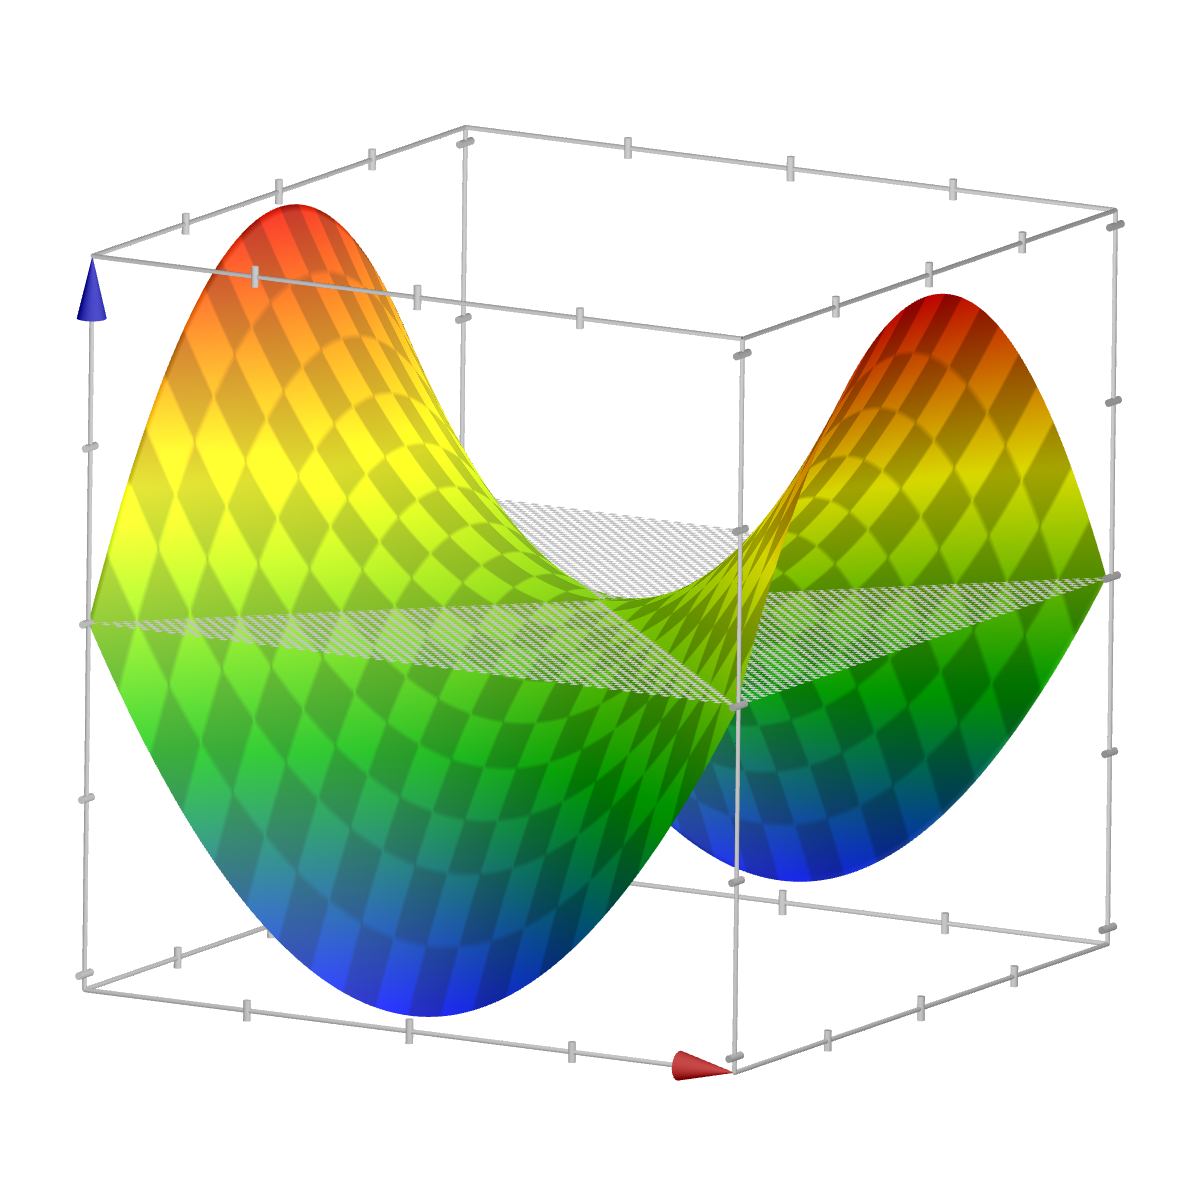
\includegraphics[keepaspectratio, scale=0.12]{figures/minimax_example.png}
        \end{center}
      \end{figure}
    \end{column}
  \end{columns}
\end{frame}

% 2. Background
% ----------------------------------------------------------------
\section{Background}

\begin{frame}{Background}
  - Georgiev and Tanaka \cite{MR1807037} extended the minimax inequality to the form of set-valued maps.
  % P. G. Georgiev と T. Tanaka によって集合値への minimax 不等式の拡張が進められた。

  - Kuwano, Tanaka, and Yamada \cite{MR2778674} constructed the result of four types set-valued minimax inequalities
  with set relations.
  % I. Kuwano と T. Tanaka, S. Yamada によって set-relations の比較にに対してスカラー関数を対応させたものの minimax 不等式の拡張が進められた。

  - Our goal is to generalize the result of four types set-valued minimax inequalities without set-relations and the scalarization functions.
  % set-relations の比較に依存しない形、またスカラー化関数がその比較に依存しない形を目指す。
\end{frame}

\begin{frame}
  \begin{block}{Theorem \cite{MR2778674}}
    Let $X$ be a nonempty compact convex subset of a Hausdorff topological vector space,
    $Y$ a real topological vector space, $C$ a proper closed convex cone in $Y$ with $\Interior{C} \ne \emptyset$
    and $F\colon X \times X \to \mathcal{P}(Y) \backslash \{\emptyset\}$ If $F$ satisfies the following conditions:
    \begin{enumerate}
      \item $F$ is $C$-bounded on $X \times X$,
      \item for each fixed $y \in X$, $F(\cdot,y)$ is $C$-lower continuous,
      \item for each fixed $x \in X$, $f(x, \cdot)$ is type (5) properly $C$-quasi concave,
      \item for all $x \in X$, $F(x,x) \subset -C$,
    \end{enumerate}
    then there exists $\bar{x} \in X$ such that $F(\bar{x},y) \subset -C$ for all $y \in X$.
  \end{block}
\end{frame}

% 3. Preliminaries
% ----------------------------------------------------------------
\section{Preliminaries}

\begin{frame}{Preliminaries}
  Let $X$ be a topological space, $Y$ a real topological vector space, and $\theta_Y$ be a zero vector in $Y$.
  Define that $\mathcal{P}(Y)$ is the set of all nonempty subsets of $Y$.
  The sets of neighborhoods of $x \in X$ and $y \in Y$ is denoted by $\mathcal{N}_X (x)$ and $\mathcal{N}_Y (y)$, respectively.

  \begin{block}{Definition \cite{500001551932}}
    Let $F \colon X \to \mathcal{P}(Y)$, $x_0 \in X$, $\preccurlyeq$ a binary relation on $\mathcal{P}(Y)$
    and $C \subset Y$ a convex cone. We say that $F$ is $(\preccurlyeq, C)$-continuous at $x_0$ if
    \begin{equation}
      \forall W \subset Y, W\:\text{open},W \preccurlyeq F(x_0), \exists V \in \mathcal{N}_{X}(x_0) \SuchThat W + C \preccurlyeq F(x), \forall x \in V. \notag
    \end{equation}
  \end{block}
\end{frame}

\begin{frame}{Preliminaries (Lower semicontinuity)}
  \begin{block}{Definition \cite{500001551932}}
    Let $\varphi \colon \mathcal{P}(Y) \to \RealNumberSet \cup \{\pm \infty\}$, $A_0 \in \mathcal{P}(Y)$,
    $\preccurlyeq$ a binary relation on $\mathcal{P}(Y)$, and $C$ a convex cone in $Y$ with $C \ne Y$. Then,
    we say that $\varphi$ is $(\preccurlyeq, C)$-lower semicontinuous at $A_0$ if
    \begin{equation}
      \forall r < \varphi (A_0), \exists W \in \mathcal{P}(Y), W\:\text{open}, \SuchThat W \preccurlyeq A_0 \:\text{and}\:
      r > \varphi (A), \forall A \in U(W + C, \preccurlyeq); \notag
    \end{equation}
    where $U(V,\preccurlyeq) \coloneqq \SetForm{A \in \mathcal{P}(Y)}{V \preccurlyeq A}$.
  \end{block}

  \begin{block}{Theorem \cite{500001551932}}
    Let $F \colon X \to \mathcal{P}(Y)$, $\varphi \colon \mathcal{P}(Y) \to \RealNumberSet \cup \{\pm \infty\}$, $x_0 \in X$,
    $\preccurlyeq$ a binary relation on $\mathcal{P}(Y)$, and $C$ a convex cone. If $F$ is $(\preccurlyeq, C)$-continuous at $x_0$
    and $\varphi$ is $(\preccurlyeq, C)$-lower semicontinuous at $F(x_0)$, then $(\varphi \circ F)$ is lower semicontinuous at $x_0$.
  \end{block}
\end{frame}

\begin{frame}{Preliminaries (Convexity)}
  \begin{block}{Definition \cite{MR3458699}}
    Let $\mathcal{A} \subset \mathcal{P}(Y) \backslash \{\emptyset\}$. $\mathcal{A}$ is said to be convex if for each $A_1, A_2 \in \mathcal{A}$ and $\lambda \in (0,1)$,
    \begin{equation}
      \lambda A_1 + (1-\lambda) A_2 \in \mathcal{A}. \notag
    \end{equation}
  \end{block}

  \begin{block}{Definition \cite{MR3458699}}
    Let $\varphi \colon \mathcal{P}(Y) \to \RealNumberSet \cup \{\pm \infty\}$. Then,
    \begin{enumerate}
      \item $\varphi$ is quasi convex if for any $\alpha \in \RealNumberSet$,
            $\OrderingLevelSets{\varphi}{\leq}{\alpha} \coloneqq \SetForm{A \in \mathcal{P}(Y) \backslash \{\emptyset\}}{\varphi(A) \leq \alpha}$ is convex.
      \item $\varphi$ is quasi concave if for any $\alpha \in \RealNumberSet$,
            $\OrderingLevelSets{\varphi}{\geq}{\alpha} \coloneqq \SetForm{A \in \mathcal{P}(Y) \backslash \{\emptyset\}}{\varphi(A) \geq \alpha}$ is convex.
    \end{enumerate}
  \end{block}
\end{frame}

\begin{frame}{Preliminaries (Convexity)}
  \begin{block}{Definition}
    Let $X$ be a nonempty set, $Y$ a real topological vector space, $C$ a convex cone in $Y$, and $F\colon X \to 2^Y \backslash \{\emptyset\}$ a set-valued map.
    \begin{enumerate}
      \item $F$ is called $(\preccurlyeq)$-naturally quasi convex if for each $x,y \in X$ and $\lambda \in (0,1)$, there exists $\mu \in [0,1]$ such that
            \begin{equation}
              F(\lambda x + (1-\lambda)y) \preccurlyeq \mu F(x) + (1-\mu) F(y). \notag
            \end{equation}
      \item $F$ is called $(\preccurlyeq)$-naturally quasi concave if for each $x,y \in X$ and $\lambda \in (0,1)$, there exists $\mu \in [0,1]$ such that
            \begin{equation}
              \mu F(x) + (1-\mu) F(y) \preccurlyeq F(\lambda x + (1-\lambda)y). \notag
            \end{equation}
    \end{enumerate}
  \end{block}
\end{frame}

% Main results
% ----------------------------------------------------------------
\section{Main results}

% 4.1
\begin{frame}{Specific scalarization function}
  To extend Ky Fan inequality for set-valued maps with a binary relation, consider assumptions of scalarization fucntions. To begin with, introduce four properties;
  \begin{enumerate}
    \item $\varphi$ is $(\preccurlyeq, C)$-lower semicontinuous,
    \item $\varphi$ is quasi concave,
    \item $\varphi$ is $(\preccurlyeq)$-monotone,
    \item $\varphi(\{\theta\}) = 0$,
  \end{enumerate}
  and define the set of functions satisfying these properties as $\Phi(\preccurlyeq, C)$. In addition, establish three vaital properties for Ky Fan inequality;
  \begin{equation}
    \varphi (A) \leq 0 \Rightarrow A \preccurlyeq \{\theta\}. \tag*{(A1)}
  \end{equation}
\end{frame}

\begin{frame}{Main results}
  \begin{block}{Theorem}
    Let $X$ be a nonempty compact convex subset of a topological vector space,
    $Y$ a real topological vector space, $\preccurlyeq$ a binary relation on $\mathcal{P}(Y)$,
    $C$ a convex cone in $Y$, $\varphi\colon \mathcal{P}(Y) \to \RealNumberSet \cup \{\pm \infty\}$,
    and $F\colon X \times X \to \mathcal{P}(Y) \backslash \{\emptyset\}$ a set-valued map.
    For the scaralization function $\varphi \in \Phi(\preccurlyeq, C)$ satisfying Assumption (A1),
    if $F$ satisfies the following conditions:
    \begin{enumerate}
      \item $(\varphi \circ F)(x,y) \in \RealNumberSet$ for all $x,y \in X$,
      \item for each fixed $y \in X$, $F(\cdot,y)$ is $(\preccurlyeq, C)$-continuous,
      \item for each fixed $x \in X$, $F(x,\cdot)$ is $(\preccurlyeq)$-naturally quasi concave,
      \item for all $x \in X$, $F(x,x) \preccurlyeq \{\theta\}$,
    \end{enumerate}
    then there exists $\bar{x} \in X$ such that $ F(\bar{x},y) \preccurlyeq \{\theta\} $ for all $y \in X$.
  \end{block}
\end{frame}

% 6. Conclusions
% ----------------------------------------------------------------
\section{Conclusion}

% 6.1
\begin{frame}{Conclusion}
  \begin{itemize}
    \item Fan-Takahashi minimax inequalitiy and beckgrounds of my consequence were introduced with an example.
    \item We gave a new result of set-valued Fan-Takahashi inequalities via scalarization  .
    \item One of the next steps is to find a scalarization function satisfying the properties $(A1)$ in $\Phi(\preccurlyeq, C)$.
  \end{itemize}
\end{frame}

% References
% ----------------------------------------------------------------
\begin{frame}[allowframebreaks]
  \printbibliography
\end{frame}

\begin{frame}
  Thank you for your listening!
\end{frame}

\begin{frame}{Theme}

  Get the source of this theme and the demo presentation from

  \begin{center}\url{github.com/matze/mtheme}\end{center}

  The theme \emph{itself} is licensed under a
  \href{http://creativecommons.org/licenses/by-sa/4.0/}{Creative Commons
    Attribution-ShareAlike 4.0 International License}.

  \begin{center}\ccbysa\end{center}
\end{frame}

\end{document}
